\chapter{High-resolution Imaging of 3C295}

% % % % % % % % % % % % % % % % % % % % % % %
\section{Aims \& Methodology}
\pg
Our aim in this section is to create a high-resolution model of 3C295, something that - as
of yet - does not exist. More specifically, we seek to create a model that will allow us to find
good phase-calibration solutions for LOFAR international baselines. While we also solve for
amplitude gains, we know that we will need to correct the total source flux in each frequency
subband as our initial spectral model is not necessarily correct.
We select 6 sub-bands out of the total LOFAR HBA bandwidth, evenly spread throughout the bandwidth as shown in Fig. \ref{fig.freqsamp}.

\pg
This approach should allow us to appropriately constrain the final spectral behaviour of our high-resolution model, once the amplitude correction is applied to ensure our model is compliant with pre-existing flux measurements for this source \citepads{arse}. [put image of source flux as function of frequency for 3c295, citing source and ideally showing position of our subbands]

\pg
Our procedure is as follows: we self-calibrate individual subbands, starting from a model
extracted from a high-resolution VLA observation of 3C295 at 8.7 GHz \citepads[cf.][]{1991AJ....101.1623P}. Once this is done,
we extract and apply a scalar flux correction factor for each subband so that the integrated flux of our 3C295 image is compatible with the existing literature at all frequencies. The resulting model is then reliable enough to calibrate our Groth Strip data using the full LOFAR array and the entire HBA bandwidth.

% % % % % % % % % % % % % % % % % % % % % % %
\section{Data Reduction}

\subsection{Data \& Observation Properties}
\pg
talk about surveys KSP tier, when observation occurred, how long, what frequency, describe subband structure of bandwidth, describe state of LOFAR and stations at the time, etc

\subsection{Calibrating the Data}
\pg
Since we plan on applying an amplitude correction based on the works of Scaife \& Heald \citep[see][]{arse}, our overriding concern is to find good phase and amplitude gain without concern for the overall scaling factor. As such, our calibration strategy consists of calibrating 6 subbands, chosen across the LOFAR bandwidth, simultaneously. The chosen subbands, and their position in the total bandwidth, are shown here:
\begin{figure}[h]
\begin{floatrow}
\ffigbox{%
  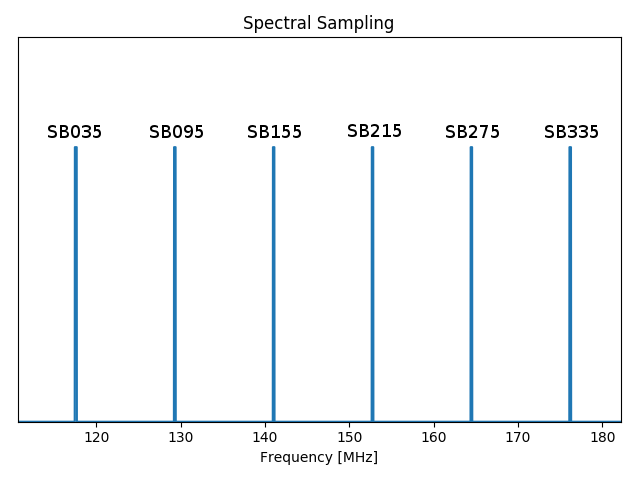
\includegraphics[width=0.5\textwidth]{images/FreqSampLabelled}
}{%
  \caption{\label{fig.freqsamp}Position of subbands chosen across full LOFAR bandwidth}%
}
\capbtabbox{%
  \begin{tabular}{|cc|} \hline
  Subband & $\nu_\mathrm{min} - \nu_\mathrm{max}$ \\ \hline
  SB035   &  117.45-117.69\\
  SB095   & 129.21-129.41\\
  SB155   & 140.93-141.12\\
  SB215   & 152.65-152.84\\
  SB275   & 164.37-164.56\\
  SB335   &  176.08-176.28 \\\hline
  \end{tabular}\vspace{1.2cm}
}{%
  \caption{Frequency bounds for the subbands chosen}%
}
\end{floatrow}
\end{figure}

\pg
Because no high-resolution models exist for 3C295 at our observing frequencies, which span quite a large bandwidth, care must be taken not to bias our model in an unphysical direction. We acquire the initial calibration model by extracting features from a NASA/IPAC Extragalactic Database\footnote{\hyperref[here]{https://ned.ipac.caltech.edu/}} image of 3C295 \citepads[see][]{1991AJ....101.1623P}, shown in Fig. \ref{fig.vla.3c295}. This feature extraction is carried out using PyBDSM \citepads{2015ascl.soft02007M}, changing all extracted Gaussians into points\footnote{This practice ensures that wrongly-estimated Gaussians do not end up introducing unphysical bias during calibration.}.
\begin{figure}[h]
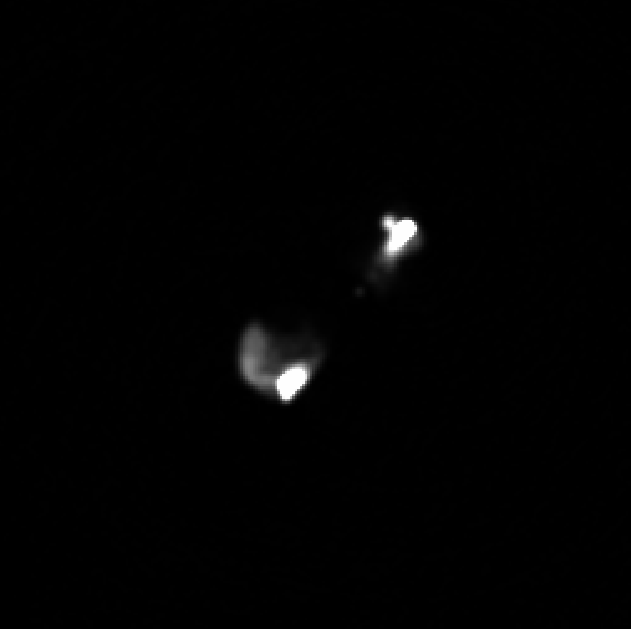
\includegraphics[width=0.4\linewidth]{images/3c295-vla}
\caption{\label{fig.vla.3c295}VLA observation of 3C295 at 8.7 GHz. Pixel size is $0.2''$.}
\end{figure}


\pg
strategy: self-cal different subbands independently across full lofar bandwidth starting with high-res VLA model
\pg
               !!! SHOW GAIN CURVES, LOTS OF PLOTS ETC
\pg
               !!! SHOW IMAGE OF WHICH SUBBANDS WE PICK ACROSS ENTIRE LOFAR BW
\pg
               !!! ANALYSE CONVERGENCE OF CALIBRATION ACROSS SUBBANDS
\pg
apply beam to account for different sensitivities of different baselines
\pg
use full-Jones solver (i.e. solve for a 2x2 complex matrix) to account for effects such as Faraday rotation etc
\pg
!!! SHOW JONES CHAIN WE SOLVE FOR AND EXPLAIN IT, MATHS ETC: $\mat{B}\mat{J}$ for Beam*Jones
\pg
!!! SHOW DIRECTION-DEPENDENT PSF EFFECT WHICH WE MODEL


% % % % % % % % % % % % % % % % % % % % % % %
\section{Overlays \& Spectral Analaysis}

\subsection{Overlays of 3C295 at Multiple Frequencies}
\pg
Show overlays of our low-freq model onto images of 3c295 at various other freqs - VLA, optical, IR, X-ray, etc.

\pg
Comment on behaviour of various components, astrometric accuracy, etc

\subsection{Spectral Analaysis}

\pg
Work with Astron guy to extract spectral behaviour of various components of 3C295 over multiple wavelengths, since he's got a purpose-built package